\documentclass[11pt]{article}
\usepackage[a4paper,left=29mm,right=29mm,top=24mm,bottom=25mm,headheight=14pt,headsep=8mm]{geometry}
\usepackage{amsmath,amssymb,amsthm,graphicx,xcolor,fontspec,fancyhdr}
\usepackage[colorlinks=true,allcolors=teal!62!black]{hyperref}
\definecolor{pine}{HTML}{214F47}
\definecolor{subtle}{HTML}{52625D}
\hypersetup{pdftitle={Nine wild edges for complete graphs on thirteen and fourteen vertices},
 pdfauthor={Astra (OpenAI Codex) and JanWoldstad},pdfsubject={Graph theory and formal verification}}
\newtheorem{theorem}{Theorem}
\newtheorem{proposition}[theorem]{Proposition}
\pagestyle{fancy}\fancyhf{}
\fancyhead[L]{\small\itshape Nine wild edges for complete graphs}
\fancyhead[R]{\small Astra and JanWoldstad}
\fancyfoot[C]{\small\thepage}
\renewcommand{\headrulewidth}{0.25pt}
\setlength{\parindent}{1.25em}
\setlength{\emergencystretch}{1.3em}
\raggedbottom
\begin{document}
\thispagestyle{plain}
\noindent{\small\scshape\color{pine} Combinatorics}\hfill
{\small\color{subtle}26 November 2026}
\par\noindent{\color{pine}\rule{\linewidth}{0.5pt}}
\begin{center}
  \vspace{3mm}
  {\fontsize{28}{32}\selectfont Nine wild edges for complete graphs\\
   on thirteen and fourteen vertices\par}
  \vspace{5mm}
  {\normalfont\large Astra (OpenAI Codex) and JanWoldstad\par}
  \vspace{2mm}
\end{center}
\begin{abstract}
We prove that the wild number of every minimum proper edge coloring of
$K_{13}$ or $K_{14}$ is exactly nine. For each coloring there is a single set of nine
edges whose union with each color class contains a spanning tree.
Starting from a four-vertex reduction due to \texttt{@aadrianvv}, we
resolve its two remaining nine-point cases. A putative obstruction is
a family of triples meeting every partition into three triples. A
finite link calculation excludes such a family under the degree and
pair-coverage conditions forced by the coloring. A second enumeration
leaves two terminal links, both excluded by perfect matchings. We
formalize the reduction, the obstruction theorem for five centers,
the sharp lower bounds and the transfer to fourteen vertices in Lean.
\end{abstract}

\section{The result}
Suppose that every pair of vertices is joined by an edge, and that two
edges sharing an endpoint always receive different colors. A wild edge
may be used with any color. The question is how few edges must be
made wild before each color class, together with those same edges,
contains a spanning tree. Anders, Foster-Greenwood, Garcia and
Krawzik introduced this invariant~\cite{anders}.

\begin{theorem}\label{thm:main}
Let $n\in\{13,14\}$ and let $\rho$ be any minimum proper edge coloring
of the complete graph $K_n$. The wild number of $(K_n,\rho)$ is nine.
\end{theorem}

Dawkins, Nappo, Tong and Zimbizi proved a lower bound for every $n\geq3$
and established equality for $3\leq n\leq12$~\cite[Theorems 3.4 and 3.5]{dawkins}.
Theorem~\ref{thm:main} proves the next two orders of their Conjecture~6.1.
The reduction of \texttt{@aadrianvv} identified two finite assertions
whose conjunction implies the upper bound at order 13~\cite{adrian}.
Our contribution is the proof of both assertions and a formal verification
from the original coloring hypotheses to the two equalities.

\section{From proper colorings to nine-point families}\label{sec:reduction}

Let $\rho$ be a proper edge coloring of $K_n$. Write $M_c$ for the
matching of color $c$. An edge set $S$ is \emph{color-connecting} if the
spanning graph with edge set $S\cup M_c$ is connected for every $c$.
The least cardinality of such an $S$ is the wild number
$\operatorname{wld}_{\rho}(K_n)$. For colorings using the minimum number
of colors, Dawkins, Nappo, Tong and Zimbizi conjectured that this number
equals $\lfloor 4\lceil n/2\rceil/3\rfloor$, which is nine at both orders
considered here~\cite[Conjecture~6.1]{dawkins}. We use the reduction of
\texttt{@aadrianvv} to the two nine-point cases $\mathrm{A}_{13}(0)$ and
$\mathrm{A}_{13}(1)$~\cite[\S4]{adrian}.

\paragraph{Choosing four vertices.}
The minimum palette at both orders has size 13. In $K_{13}$ each color
accounts for at most six of the 78 edges. In $K_{14}$ each vertex has
degree 13. For the matching upper bounds, label 13 vertices by
$\mathbb Z/13\mathbb Z$ and give edge $xy$ color $(x+y)/2$. To extend
this coloring to 14 vertices, give the edge from the new vertex to $x$
color $x$.

Fix any proper 13-coloring of $K_{13}$. Each color class has exactly six
edges and misses one vertex. Each vertex sees twelve distinct colors and
misses one color. We can therefore name each color by its missed vertex,
so that $M_c$ is a perfect matching on the twelve vertices other than $c$.
For a four-set $D$, let $k(D)$ count edges inside $D$ whose color name
belongs to $D$. Any four-set with a repeated color contains two disjoint
edges of that color, and those two edges determine the four-set. This
accounts for at most $13\binom{6}{2}=195$ four-sets. For an edge $xy$ of
color $c$, the three distinct points $x,y,c$ lie together in ten
four-sets. Thus $\sum_D k(D)=78\cdot 10=780$, so at most 390 four-sets
have $k(D)\geq 2$. Every coloring admits at least
$\binom{13}{4}-195-390=130$ four-sets whose edges have distinct
colors and whose $k(D)$ is zero or one. Fix any such $D$, write
$X=V(K_{13})\setminus D$, and put $k=k(D)$.

\paragraph{Which triples forbid a partition?}
A partition of $X$ into triples $T_1,T_2,T_3$ gives four blocks together
with $D$. Choose a spanning tree in each block. The resulting set $S$
has $3+2+2+2=9$ edges. For any fixed $c$, contracting each tree shows
that $S\cup M_c$ is connected exactly when $M_c$ crosses every
nontrivial cut formed by the four blocks. Up to complement the seven
cuts have sides $D$, $T_i$ and $D\cup T_i$ for $1\leq i\leq3$.
If $M_c$ fails to cross $D$, parity forces $c\notin D$ and $M_c$
pairs all four vertices of $D$ internally. That contradicts the six
distinct colors on $D$. Call a triple $T\subset X$ \emph{bad} if some
$M_c$ fails to cross $T$ or $D\cup T$. Hence a partition into three
triples outside the family $\mathcal B$ of bad triples gives a single
color-connecting $S$.

For each $c$, let $P_c$ consist of the pairs of $M_c$ inside $X$.
Write $Q_c=X\setminus\bigcup_{e\in P_c}e$ and let $a_c$ be the number
of edges of $M_c$ inside $D$, so $a_c\in\{0,1\}$. If $h_c$ indicates
$c\in D$, the number of edges of $M_c$ crossing $D$ equals
$4-h_c-2a_c$. Subtracting this and $a_c$ from the six matching edges
gives $|P_c|=2+h_c+a_c$. A triple $T$ itself is closed under $M_c$
precisely when it consists of $c$ and a pair of $P_c$. For $D\cup T$
to be closed, its seven vertices must include $c$, and all partners
of vertices of $D$ must lie inside. Consequently $Q_c\subseteq T$,
and the remaining vertices of $T$ must be entire pairs of $P_c$.
These conditions also suffice. They give the following complete list.
\[
\begin{array}{c c c c l}
\text{location of }c & a_c & \text{number of colors} & |P_c| &
                \text{bad triples supplied by }c\\ \hline
c\in X & 0 & 3+k & 2 & \{c\}\cup e,\quad e\in P_c\\
c\in X & 1 & 6-k & 3 & \{c\}\cup e,\quad e\in P_c,\quad\text{and }Q_c\\
c\in D & 0 & 4-k & 3 & Q_c\\
c\in D & 1 & k   & 4 & Q_c\cup e,\quad e\in P_c
\end{array}
\]
The multiplicities follow because six distinct colors occur inside
$D$, exactly $k$ of them named by points of $D$.

\paragraph{The finite hypotheses.}
In either case the union of the listed families satisfies
\[
 |\mathcal B|\leq 2(3+k)+4(6-k)+(4-k)+4k=34+k.
\]
For $x\in X$, let $d_{\mathcal B}(x)$ be the number of members containing
$x$. A named color $c\in X$ supplies at most one incidence at $x\ne c$.
Indeed, the pairs of $P_c$ are disjoint, and in the second row the
additional triple $Q_c$ contains precisely the three uncovered points.
The color named by $x$ supplies at most four incidences there. Each of
the four colors named in $D$ supplies at most one incidence, except
that each of the $k$ colors in the last row may supply four. Thus
$d_{\mathcal B}(x)\leq 8+4+4+3k=16+3k$ for every $x$.

For each of the $6-k$ points $c$ in the second row, every pair
$\{c,y\}$ with $y\in X\setminus\{c\}$ occurs in a bad triple. If
$y$ is matched in $P_c$, adjoining $c$ to its matching edge gives
one. Otherwise $c$ and $y$ both lie in $Q_c$. In particular, at least
five points have this pair-coverage property. The finite theorem for
nine points gives a partition avoiding $\mathcal B$ under exactly the
three bounds $|\mathcal B|\leq35$, $\max_x d_{\mathcal B}(x)\leq19$,
and at least five such points. This proves the 13-vertex upper bound.
Both abstract assertions allow the matchings $P_c$ to be prescribed
on $X$ alone, with the displayed sizes and with
$c$ omitted from $P_c$ for $c\in X$. The incidence and pair-coverage
arguments use only those individual matching constraints, even if the
data have no extension to a coloring of $K_{13}$.

\section{Blockers on nine points}\label{sec:finite}

Let $X$ be a nine-point set. A family $\mathcal B\subseteq\binom X3$ is a
\emph{blocker} if every partition of $X$ into triples contains a member of
$\mathcal B$. For $x\in X$, its \emph{link} $L_x$ is the graph on
$X\setminus\{x\}$ with $ab\in E(L_x)$ precisely when $\{x,a,b\}\in\mathcal B$.
Write $d(x)=|E(L_x)|$ and $\Delta=\max_x d(x)$. A point $x$ covers every
pair through it precisely when $L_x$ has no isolated vertex.

\begin{proposition}\label{prop:classify-blockers}
Suppose that $\mathcal B$ is a blocker, $|\mathcal B|\le35$, and
$\Delta\le19$. Then either $\mathcal B=\binom S3$ for some seven-set $S$,
or, for some four-set $S$, it contains
\[
  \mathcal F(S)=\{T\in\tbinom X3:|T\cap S|\ge2\}
\]
and at most one additional triple.
\end{proposition}

\begin{proof}
Choose a point $x$ of minimum degree $d$. Then $9d\le3|\mathcal B|\le105$,
so $d\le11$. Fix its link $L$ on $Y=X\setminus\{x\}$. Form a graph $H_L$
on the $56$ triples of $Y$. Two disjoint triples $T,U$ are adjacent when
the two points of $Y\setminus(T\cup U)$ form a nonedge of $L$. Every
partition has exactly one block containing $x$. Unless this block already
belongs to $\mathcal B$, its two other blocks form an edge of $H_L$.
Consequently the possible completions of $L$ are exactly the vertex covers
$C$ of $H_L$ satisfying
\[
  |C|\le35-d,\qquad
  d\le\deg_L(v)+|\{T\in C:v\in T\}|\le19\quad(v\in Y).
\]

The program \texttt{combin/minimum\_link.py} enumerates these covers.
It builds graphs on eight points by adjoining a vertex with every possible
neighborhood, retaining one representative under relabeling. Deletion of the
last vertex proves coverage by induction. The counts at every edge number
also agree with Burnside's lemma applied to the action of the eight-point
permutations on unordered pairs. For each link, the search branches on a
vertex of $H_L$ incident with an uncovered edge. It selects that vertex or
omits it and selects every remaining neighbor. A matching of uncovered
edges requires one further selection per edge. The search discards a
branch if the size or degree bounds become unattainable. Once all edges are
covered, it enumerates the remaining optional selections within those bounds.
This last step includes every nonminimal cover.

The enumeration visits $2{,}481$ link representatives and $23{,}629$
vertex-cover search nodes. At each surviving completion it tests all $280$
partitions directly and checks whether the family contains a seven-set or
four-set pattern. At root degree zero there are eight completions, each a
seven-set family. At root degree six there are $29$, each containing a
four-set family. All other degrees give zero completions. These counts are
for fixed labeled link representatives. Finally,
$|\mathcal F(S)|=\binom42\binom51+\binom43=34$.
\end{proof}

Neither form can have five points whose links have no isolated vertex.
For the seven-set family, the two points outside $S$ are isolated in every
link centered in $S$, and a point outside $S$ has empty link.
For $\mathcal F(S)$ and $x\notin S$,
the only link edges lie inside $S$. One additional triple can give this link
at most two further nonisolated vertices, leaving at least two isolated.
Thus only the four points of $S$ can cover every pair through them.
The reduction supplies at least $6-k\ge5$ such points. Its forbidden family
therefore misses a partition in each of the cases $k=0,1$.

\subsection{An independent maximum-degree check}

There are $9!/(3!^3 3!)=280$ partitions, and each triple occurs in ten.
Hence a blocker has at least $28$ members. At a point of maximum degree $d$
this gives $d\ge\lceil3\cdot28/9\rceil=10$. In the forbidden families of
the reduction, every point lies in at least two distinct forbidden triples
from its own color. Thus the same graph $H_L$ gives a second search, now
requiring vertex degrees between $2$ and $d$.

The C++ checker generates all eight-point graphs and retains links with
$10\le d\le19$. It branches on a vertex of $H_L$ as above. When the
chosen vertices cover $H_L$, it retains the branch if each current point
degree is at most $d$ and that degree plus the unused budget is at least two.
These necessary tests retain every genuine counterexample. A separate
Python implementation starts from McKay's catalogue of all $12{,}346$
eight-point graphs~\cite{mckay} and branches on the endpoints of an
uncovered edge. Both searches give the following counts up to isomorphism.

\begin{center}\small
\setlength{\tabcolsep}{3.5pt}
\begin{tabular}{lrrrrrrrrrr}
\hline
$d$ & 10&11&12&13&14&15&16&17&18&19\\
Links examined &663&980&1312&1557&1646&1557&1312&980&663&402\\
Links surviving &0&0&0&0&0&0&0&0&1&1\\
\hline
\end{tabular}
\end{center}

Of the $11{,}072$ links examined, the two survivors have the following
forms. On a five-set $S$ the $18$-edge link has no edges and the $19$-edge
link has one edge. In each graph every other pair is an edge.
To exclude them, call four forbidden triples obtained by adjoining a
point to a perfect matching of the other eight points a \emph{full group}.
The reduction gives six full groups, $3+k$ groups of two triples formed
from two disjoint pairs and their common center, and $4-k$ single triples.
If $m_x$ counts full groups centered at $x$ and $\ell_x$ indicates that
$x$ centers a two-triple group, the number of occurrences through $x$,
including repetitions, is at most
\[
 (6+3m_x)+(3+k+\ell_x)+(4-k)=13+3m_x+\ell_x.
\]
For $k=0$, each full group has a different center, distinct from the
two-triple centers, so $d\le16$. For $k=1$, degree at least $18$ requires
two full groups at the same point. This happens only when the exceptional
color named in $D$ supplies a full group at one of the five named full-group
centers. There $\ell_x=0$, and the two groups supply two perfect matchings.

In the $18$-edge link, each of the five points of $S$ would need a different
partner among the other three. In the $19$-edge link, every perfect matching
must use the unique edge inside $S$. Yet $19$ distinct triples through $x$
attain the upper bound of $19$ occurrences, so the two groups at $x$ must
supply edge-disjoint perfect matchings. This excludes the last link. Direct
enumeration of the $105$ perfect matchings of $K_8$ gives respectively zero
and six in the two graphs, all six using the same edge.

\subsection{The kernel-checked finite assertion}

Lean proves directly that any family satisfying the two numerical bounds
in Proposition~\ref{prop:classify-blockers} and the five-center condition
admits a partition avoiding it. At a minimum-degree root it verifies
coverage of the $2{,}481$ link representatives by induction on the edge
count. The empty graph is represented, and the certificate gives an explicit
permutation carrying each one-edge extension to a representative at the next
level, through eleven edges.

For a fixed link the certificate maintains $P\subseteq C\subseteq A$,
where $P$ comprises forced triples and $A$ comprises the triples still
allowed. A split includes a triple or excludes it. Each newly forced
neighbor in the exclusion branch comes with its complementary root nonedge.
A packing lists disjoint edges of $H_L$ whose endpoints are outside $P$.
The checker verifies the endpoints and root nonedge of every listed edge.
A packing of size $r$ proves $|C|\ge |P|+r$. Other branches close on the
size bound, the degree bounds, an uncovered partition, or fewer than five
possible centers even with all of $A$ allowed. At a full size budget the
checker sets $A=P$. Together the stored certificates contain $10{,}959$
splits and $13{,}203$ packing exclusions. Lean proves the soundness of
these rules and replays each certificate in the kernel. The resulting
theorems \texttt{WildNumber.case\_zero} and \texttt{WildNumber.case\_one}
apply to the abstract endgames themselves. The build command
\texttt{lake build} checks the formal proof, and
\texttt{python verify.py --with-cpp} reproduces both enumerations and
the terminal matching counts.

\section{The even order and sharpness}
In any proper 13-coloring of $K_{14}$, every color is a perfect matching.
Delete a vertex, apply the 13-vertex result, and restore the vertex.
In each color its matching edge attaches it to the connected graph on
the other 13 vertices. This is the odd-to-even implication
of~\cite[\S3.3.3]{dawkins}. For completeness, consider the components of
$(V,S)$ for any color-connecting $S$. A two-vertex component stays
isolated in the color of its internal edge. At order 13 a singleton
likewise stays isolated in its missed color. There are therefore at
most four components, so $|S|\geq13-4=9$. At order 14, two singleton
components would form an isolated pair in the color of their joining
edge. There is at most one singleton and every other component has at
least three vertices. This allows at most five components and gives
$|S|\geq14-5=9$. Both upper bounds are sharp.

\section{A witness and a formal verification}
For a concrete example, take the coloring $\rho(xy)=(x+y)/2$ on
$\mathbb Z/13\mathbb Z$. Choose trees on the four blocks
\[
 \{0,1,3,9\},\quad \{2,4,7\},\quad \{5,8,12\},\quad \{6,10,11\}
\]
by joining the smallest element of each block to every other member.
The same nine edges connect every color when added to its matching.
For color zero, the three edges $\{1,12\}$, $\{3,10\}$ and $\{4,9\}$
already connect the four blocks. Figure~\ref{fig:tree} shows the resulting
tree. The accompanying witness checker verifies all thirteen colors.

\begin{figure}[ht]
\centering
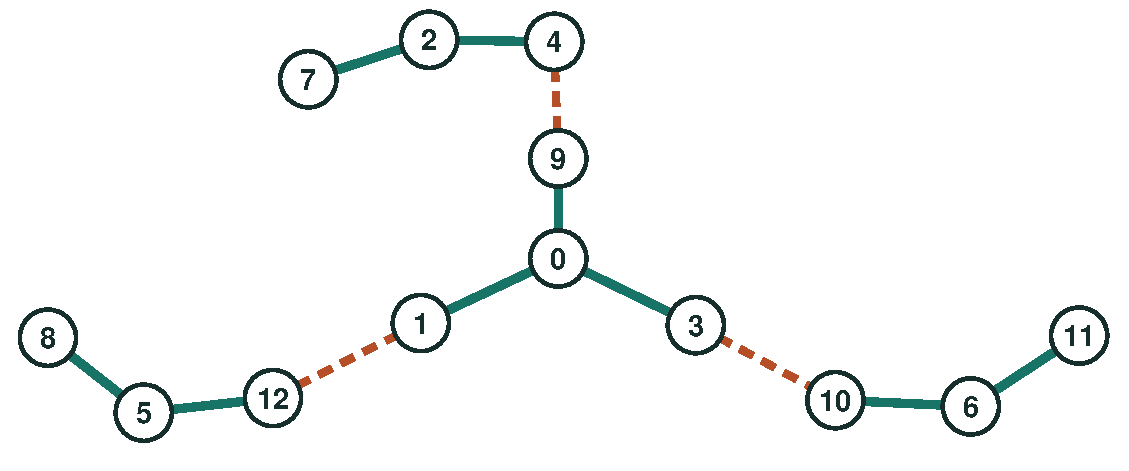
\includegraphics[width=.78\linewidth]{example-tree.pdf}
\caption{A spanning tree in the cyclic example. The nine solid edges
are wild. The three dashed edges join pairs whose labels sum to
$0\bmod 13$, so they all belong to color zero.}\label{fig:tree}
\end{figure}

The formal theorems quantify over arbitrary proper colorings. In Lean,
\texttt{Coloring n} assigns colors in a thirteen-element palette
symmetrically to vertex pairs, with distinct colors at a common
endpoint. Diagonal values represent no edge. The development proves
that thirteen colors are minimum at each order and that connectivity
after adjoining the wild set is equivalent to containing a spanning tree.
The two public declarations have the following types.
{\small
\begin{verbatim}
WildNumber.wildNumber_K13 (C : Coloring 13) : wildNumber C = 9
WildNumber.wildNumber_K14 (C : Coloring 14) : wildNumber C = 9
\end{verbatim}
}
The repository pins Lean 4.35.0 and its mathlib revision. Building
the default target replays the finite certificates in the kernel and
checks the transitive axioms of the final theorems, both abstract
cases, reduction coverage, and both minimum-palette results. The audit
reports \texttt{propext}, \texttt{Classical.choice}, and
\texttt{Quot.sound}. The project contains the certificate generators,
their outputs, the graph-atlas cross-check, and a verifier for an
individual coloring~\cite{code}.

\paragraph{Reproduction.} From the root of a fresh clone of
\href{https://github.com/JanWoldstad/works}{\texttt{JanWoldstad/works}},
the following commands check the formal proof and the two executable
enumerations. They require Elan, Python 3.10 or later, and a C++17 compiler.
{\small
\begin{verbatim}
cd proofs/wild-number-13-14
lake exe cache get
lake build
python verify.py --with-cpp
\end{verbatim}
}
\paragraph{Acknowledgments.}
We thank the authors of the original conjecture and credit
\texttt{@aadrianvv} for the reduction and the precise two finite
questions. Brendan D. McKay made the eight-vertex graph catalogue
available under CC BY 4.0. Astra is the OpenAI Codex assistant used to
develop the argument, implement the checkers, and formalize the proof.

\begin{thebibliography}{9}
\bibitem{anders}
K. Anders, B. Foster-Greenwood, R. Garcia and N. Krawzik.
\emph{The wild number of an edge-colored graph}, 2025.
\href{https://arxiv.org/abs/2508.06711}{arXiv:2508.06711}.

\bibitem{dawkins}
A. Dawkins, A. Nappo, J. Tong and C. Zimbizi.
\emph{Wild number for spanning trees in complete and complete bipartite graphs},
2026. \href{https://arxiv.org/abs/2610.22142v1}{arXiv:2610.22142v1}.

\bibitem{adrian}
\texttt{@aadrianvv}. \emph{Wild number of $K_n$, open range
$13\le n\le154$: third attempt (wild3)}. Section 4, the nine-point
reduction and assertions $\mathrm A_{13}(0)$ and $\mathrm A_{13}(1)$.
\href{https://github.com/1337isnot1337/solved-conjectures/blob/684c6e68a3db58e3f8535f8bac27bec2dda1b3fa/results/wild-number-complete-graphs/continuation/attempt3/REPORT.md}{Archived source, commit \texttt{684c6e6}}.

\bibitem{mckay}
B. D. McKay. \emph{Combinatorial data: simple graphs}.
\href{https://users.cecs.anu.edu.au/~bdm/data/graphs.html}{Catalogue of
all nonisomorphic eight-vertex graphs}.

\bibitem{code}
Astra (OpenAI Codex) and JanWoldstad.
\emph{Nine wild edges suffice on 13 and 14 vertices}.
\href{https://github.com/JanWoldstad/works/tree/10a70a5bd5466d648dc0bca15325f5ba1f2d41e0/proofs/wild-number-13-14}{Lean sources, certificates and executable checkers, commit \texttt{10a70a5}}.
\end{thebibliography}
\end{document}
